\documentclass[1p]{elsarticle_modified}
%\bibliographystyle{elsarticle-num}

%\usepackage[colorlinks]{hyperref}
%\usepackage{abbrmath_seonhwa} %\Abb, \Ascr, \Acal ,\Abf, \Afrak
\usepackage{amsfonts}
\usepackage{amssymb}
\usepackage{amsmath}
\usepackage{amsthm}
\usepackage{scalefnt}
\usepackage{amsbsy}
\usepackage{kotex}
\usepackage{caption}
\usepackage{subfig}
\usepackage{color}
\usepackage{graphicx}
\usepackage{xcolor} %% white, black, red, green, blue, cyan, magenta, yellow
\usepackage{float}
\usepackage{setspace}
\usepackage{hyperref}

\usepackage{tikz}
\usetikzlibrary{arrows}

\usepackage{multirow}
\usepackage{array} % fixed length table
\usepackage{hhline}

%%%%%%%%%%%%%%%%%%%%%
\makeatletter
\renewcommand*\env@matrix[1][\arraystretch]{%
	\edef\arraystretch{#1}%
	\hskip -\arraycolsep
	\let\@ifnextchar\new@ifnextchar
	\array{*\c@MaxMatrixCols c}}
\makeatother %https://tex.stackexchange.com/questions/14071/how-can-i-increase-the-line-spacing-in-a-matrix
%%%%%%%%%%%%%%%

\usepackage[normalem]{ulem}

\newcommand{\msout}[1]{\ifmmode\text{\sout{\ensuremath{#1}}}\else\sout{#1}\fi}
%SOURCE: \msout is \stkout macro in https://tex.stackexchange.com/questions/20609/strikeout-in-math-mode

\newcommand{\cancel}[1]{
	\ifmmode
	{\color{red}\msout{#1}}
	\else
	{\color{red}\sout{#1}}
	\fi
}

\newcommand{\add}[1]{
	{\color{blue}\uwave{#1}}
}

\newcommand{\replace}[2]{
	\ifmmode
	{\color{red}\msout{#1}}{\color{blue}\uwave{#2}}
	\else
	{\color{red}\sout{#1}}{\color{blue}\uwave{#2}}
	\fi
}

\newcommand{\Sol}{\mathcal{S}} %segment
\newcommand{\D}{D} %diagram
\newcommand{\A}{\mathcal{A}} %arc


%%%%%%%%%%%%%%%%%%%%%%%%%%%%%5 test

\def\sl{\operatorname{\textup{SL}}(2,\Cbb)}
\def\psl{\operatorname{\textup{PSL}}(2,\Cbb)}
\def\quan{\mkern 1mu \triangleright \mkern 1mu}

\theoremstyle{definition}
\newtheorem{thm}{Theorem}[section]
\newtheorem{prop}[thm]{Proposition}
\newtheorem{lem}[thm]{Lemma}
\newtheorem{ques}[thm]{Question}
\newtheorem{cor}[thm]{Corollary}
\newtheorem{defn}[thm]{Definition}
\newtheorem{exam}[thm]{Example}
\newtheorem{rmk}[thm]{Remark}
\newtheorem{alg}[thm]{Algorithm}

\newcommand{\I}{\sqrt{-1}}
\begin{document}

%\begin{frontmatter}
%
%\title{Boundary parabolic representations of knots up to 8 crossings}
%
%%% Group authors per affiliation:
%\author{Yunhi Cho} 
%\address{Department of Mathematics, University of Seoul, Seoul, Korea}
%\ead{yhcho@uos.ac.kr}
%
%
%\author{Seonhwa Kim} %\fnref{s_kim}}
%\address{Center for Geometry and Physics, Institute for Basic Science, Pohang, 37673, Korea}
%\ead{ryeona17@ibs.re.kr}
%
%\author{Hyuk Kim}
%\address{Department of Mathematical Sciences, Seoul National University, Seoul 08826, Korea}
%\ead{hyukkim@snu.ac.kr}
%
%\author{Seokbeom Yoon}
%\address{Department of Mathematical Sciences, Seoul National University, Seoul, 08826,  Korea}
%\ead{sbyoon15@snu.ac.kr}
%
%\begin{abstract}
%We find all boundary parabolic representation of knots up to 8 crossings.
%
%\end{abstract}
%\begin{keyword}
%    \MSC[2010] 57M25 
%\end{keyword}
%
%\end{frontmatter}

%\linenumbers
%\tableofcontents
%
\newcommand\colored[1]{\textcolor{white}{\rule[-0.35ex]{0.8em}{1.4ex}}\kern-0.8em\color{red} #1}%
%\newcommand\colored[1]{\textcolor{white}{ #1}\kern-2.17ex	\textcolor{white}{ #1}\kern-1.81ex	\textcolor{white}{ #1}\kern-2.15ex\color{red}#1	}

{\Large $\underline{12a_{0591}~(K12a_{0591})}$}

\setlength{\tabcolsep}{10pt}
\renewcommand{\arraystretch}{1.6}
\vspace{1cm}\begin{tabular}{m{100pt}>{\centering\arraybackslash}m{274pt}}
\multirow{5}{120pt}{
	\centering
	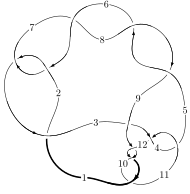
\includegraphics[width=112pt]{../../../GIT/diagram.site/Diagrams/png/1392_12a_0591.png}\\
\ \ \ A knot diagram\footnotemark}&
\allowdisplaybreaks
\textbf{Linearized knot diagam} \\
\cline{2-2}
 &
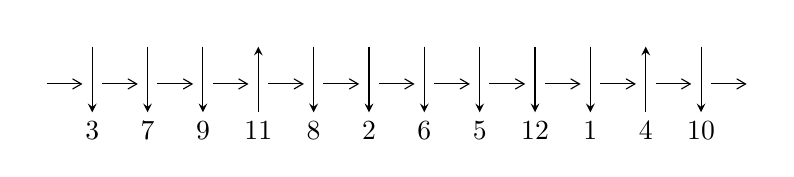
\begin{tikzpicture}[x=20pt, y=17pt]
	% nodes
	\node (C0) at (0, 0) {};
	\node (C1) at (1, 0) {};
	\node (C1U) at (1, +1) {};
	\node (C1D) at (1, -1) {3};

	\node (C2) at (2, 0) {};
	\node (C2U) at (2, +1) {};
	\node (C2D) at (2, -1) {7};

	\node (C3) at (3, 0) {};
	\node (C3U) at (3, +1) {};
	\node (C3D) at (3, -1) {9};

	\node (C4) at (4, 0) {};
	\node (C4U) at (4, +1) {};
	\node (C4D) at (4, -1) {11};

	\node (C5) at (5, 0) {};
	\node (C5U) at (5, +1) {};
	\node (C5D) at (5, -1) {8};

	\node (C6) at (6, 0) {};
	\node (C6U) at (6, +1) {};
	\node (C6D) at (6, -1) {2};

	\node (C7) at (7, 0) {};
	\node (C7U) at (7, +1) {};
	\node (C7D) at (7, -1) {6};

	\node (C8) at (8, 0) {};
	\node (C8U) at (8, +1) {};
	\node (C8D) at (8, -1) {5};

	\node (C9) at (9, 0) {};
	\node (C9U) at (9, +1) {};
	\node (C9D) at (9, -1) {12};

	\node (C10) at (10, 0) {};
	\node (C10U) at (10, +1) {};
	\node (C10D) at (10, -1) {1};

	\node (C11) at (11, 0) {};
	\node (C11U) at (11, +1) {};
	\node (C11D) at (11, -1) {4};

	\node (C12) at (12, 0) {};
	\node (C12U) at (12, +1) {};
	\node (C12D) at (12, -1) {10};
	\node (C13) at (13, 0) {};

	% arrows
	\draw[->,>={angle 60}]
	(C0) edge (C1) (C1) edge (C2) (C2) edge (C3) (C3) edge (C4) (C4) edge (C5) (C5) edge (C6) (C6) edge (C7) (C7) edge (C8) (C8) edge (C9) (C9) edge (C10) (C10) edge (C11) (C11) edge (C12) (C12) edge (C13) ;	\draw[->,>=stealth]
	(C1U) edge (C1D) (C2U) edge (C2D) (C3U) edge (C3D) (C4D) edge (C4U) (C5U) edge (C5D) (C6U) edge (C6D) (C7U) edge (C7D) (C8U) edge (C8D) (C9U) edge (C9D) (C10U) edge (C10D) (C11D) edge (C11U) (C12U) edge (C12D) ;
	\end{tikzpicture} \\
\hhline{~~} \\& 
\textbf{Solving Sequence} \\ \cline{2-2} 
 &
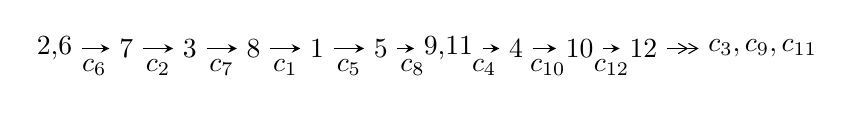
\begin{tikzpicture}[x=23pt, y=7pt]
	% node
	\node (A0) at (-1/8, 0) {2,6};
	\node (A1) at (1, 0) {7};
	\node (A2) at (2, 0) {3};
	\node (A3) at (3, 0) {8};
	\node (A4) at (4, 0) {1};
	\node (A5) at (5, 0) {5};
	\node (A6) at (97/16, 0) {9,11};
	\node (A7) at (57/8, 0) {4};
	\node (A8) at (65/8, 0) {10};
	\node (A9) at (73/8, 0) {12};
	\node (C1) at (1/2, -1) {$c_{6}$};
	\node (C2) at (3/2, -1) {$c_{2}$};
	\node (C3) at (5/2, -1) {$c_{7}$};
	\node (C4) at (7/2, -1) {$c_{1}$};
	\node (C5) at (9/2, -1) {$c_{5}$};
	\node (C6) at (11/2, -1) {$c_{8}$};
	\node (C7) at (53/8, -1) {$c_{4}$};
	\node (C8) at (61/8, -1) {$c_{10}$};
	\node (C9) at (69/8, -1) {$c_{12}$};
	\node (A10) at (11, 0) {$c_{3},c_{9},c_{11}$};

	% edge
	\draw[->,>=stealth]	
	(A0) edge (A1) (A1) edge (A2) (A2) edge (A3) (A3) edge (A4) (A4) edge (A5) (A5) edge (A6) (A6) edge (A7) (A7) edge (A8) (A8) edge (A9) ;
	\draw[->>,>={angle 60}]	
	(A9) edge (A10);
\end{tikzpicture} \\ 

\end{tabular} \\

\footnotetext{
The image of knot diagram is generated by the software ``\textbf{Draw programme}" developed by Andrew Bartholomew(\url{http://www.layer8.co.uk/maths/draw/index.htm\#Running-draw}), where we modified some parts for our purpose(\url{https://github.com/CATsTAILs/LinksPainter}).
}\phantom \\ \newline 
\centering \textbf{Ideals for irreducible components\footnotemark of $X_{\text{par}}$} 
 
\begin{align*}
I^u_{1}&=\langle 
2 u^{58}-4 u^{57}+\cdots+b+2,\;- u^{58}+3 u^{57}+\cdots+a-3,\;u^{59}-2 u^{58}+\cdots+6 u^2-1\rangle \\
I^u_{2}&=\langle 
- u^2+b,\;u^4+a- u+1,\;u^5+u^4- u^2+u+1\rangle \\
\\
\end{align*}
\raggedright * 2 irreducible components of $\dim_{\mathbb{C}}=0$, with total 64 representations.\\
\footnotetext{All coefficients of polynomials are rational numbers. But the coefficients are sometimes approximated in decimal forms when there is not enough margin.}
\newpage
\renewcommand{\arraystretch}{1}
\centering \section*{I. $I^u_{1}= \langle 2 u^{58}-4 u^{57}+\cdots+b+2,\;- u^{58}+3 u^{57}+\cdots+a-3,\;u^{59}-2 u^{58}+\cdots+6 u^2-1 \rangle$}
\flushleft \textbf{(i) Arc colorings}\\
\begin{tabular}{m{7pt} m{180pt} m{7pt} m{180pt} }
\flushright $a_{2}=$&$\begin{pmatrix}0\\u\end{pmatrix}$ \\
\flushright $a_{6}=$&$\begin{pmatrix}1\\0\end{pmatrix}$ \\
\flushright $a_{7}=$&$\begin{pmatrix}1\\u^2\end{pmatrix}$ \\
\flushright $a_{3}=$&$\begin{pmatrix}- u\\- u^3+u\end{pmatrix}$ \\
\flushright $a_{8}=$&$\begin{pmatrix}- u^2+1\\u^2\end{pmatrix}$ \\
\flushright $a_{1}=$&$\begin{pmatrix}u^3\\u^5- u^3+u\end{pmatrix}$ \\
\flushright $a_{5}=$&$\begin{pmatrix}u^4- u^2+1\\- u^4\end{pmatrix}$ \\
\flushright $a_{9}=$&$\begin{pmatrix}- u^6+u^4-2 u^2+1\\u^6+u^2\end{pmatrix}$ \\
\flushright $a_{11}=$&$\begin{pmatrix}u^{58}-3 u^{57}+\cdots+8 u+3\\-2 u^{58}+4 u^{57}+\cdots-2 u-2\end{pmatrix}$ \\
\flushright $a_{4}=$&$\begin{pmatrix}u^{15}-2 u^{13}+6 u^{11}-8 u^9+10 u^7-8 u^5+4 u^3-2 u\\- u^{15}+u^{13}-4 u^{11}+3 u^9-4 u^7+2 u^5-2 u^3+u\end{pmatrix}$ \\
\flushright $a_{10}=$&$\begin{pmatrix}u^{58}-2 u^{57}+\cdots+7 u+2\\- u^{58}+2 u^{57}+\cdots-2 u-1\end{pmatrix}$ \\
\flushright $a_{12}=$&$\begin{pmatrix}u^{58}- u^{57}+\cdots+6 u+2\\- u^{56}+6 u^{54}+\cdots-5 u^2- u\end{pmatrix}$\\&\end{tabular}
\flushleft \textbf{(ii) Obstruction class $= -1$}\\~\\
\flushleft \textbf{(iii) Cusp Shapes $= 6 u^{58}-9 u^{57}+\cdots+11 u-4$}\\~\\
\newpage\renewcommand{\arraystretch}{1}
\flushleft \textbf{(iv) u-Polynomials at the component}\newline \\
\begin{tabular}{m{50pt}|m{274pt}}
Crossings & \hspace{64pt}u-Polynomials at each crossing \\
\hline $$\begin{aligned}c_{1},c_{5},c_{7}\\c_{8}\end{aligned}$$&$\begin{aligned}
&u^{59}+12 u^{58}+\cdots+12 u+1
\end{aligned}$\\
\hline $$\begin{aligned}c_{2},c_{6}\end{aligned}$$&$\begin{aligned}
&u^{59}-2 u^{58}+\cdots+6 u^2-1
\end{aligned}$\\
\hline $$\begin{aligned}c_{3}\end{aligned}$$&$\begin{aligned}
&u^{59}-2 u^{58}+\cdots+770 u-769
\end{aligned}$\\
\hline $$\begin{aligned}c_{4},c_{11}\end{aligned}$$&$\begin{aligned}
&u^{59}- u^{58}+\cdots-160 u-32
\end{aligned}$\\
\hline $$\begin{aligned}c_{9},c_{10},c_{12}\end{aligned}$$&$\begin{aligned}
&u^{59}-6 u^{58}+\cdots+6 u-1
\end{aligned}$\\
\hline
\end{tabular}\\~\\
\newpage\renewcommand{\arraystretch}{1}
\flushleft \textbf{(v) Riley Polynomials at the component}\newline \\
\begin{tabular}{m{50pt}|m{274pt}}
Crossings & \hspace{64pt}Riley Polynomials at each crossing \\
\hline $$\begin{aligned}c_{1},c_{5},c_{7}\\c_{8}\end{aligned}$$&$\begin{aligned}
&y^{59}+72 y^{58}+\cdots+524 y^2-1
\end{aligned}$\\
\hline $$\begin{aligned}c_{2},c_{6}\end{aligned}$$&$\begin{aligned}
&y^{59}-12 y^{58}+\cdots+12 y-1
\end{aligned}$\\
\hline $$\begin{aligned}c_{3}\end{aligned}$$&$\begin{aligned}
&y^{59}-12 y^{58}+\cdots+8725844 y-591361
\end{aligned}$\\
\hline $$\begin{aligned}c_{4},c_{11}\end{aligned}$$&$\begin{aligned}
&y^{59}+33 y^{58}+\cdots-512 y-1024
\end{aligned}$\\
\hline $$\begin{aligned}c_{9},c_{10},c_{12}\end{aligned}$$&$\begin{aligned}
&y^{59}-56 y^{58}+\cdots+38 y-1
\end{aligned}$\\
\hline
\end{tabular}\\~\\
\newpage\flushleft \textbf{(vi) Complex Volumes and Cusp Shapes}
$$\begin{array}{c|c|c}  
\text{Solutions to }I^u_{1}& \I (\text{vol} + \sqrt{-1}CS) & \text{Cusp shape}\\
 \hline 
\begin{aligned}
u &= -0.927503 + 0.362332 I \\
a &= \phantom{-}1.043690 + 0.616352 I \\
b &= -0.037342 - 1.128440 I\end{aligned}
 & -8.68686 - 0.29443 I & -15.0428 - 2.5911 I \\ \hline\begin{aligned}
u &= -0.927503 - 0.362332 I \\
a &= \phantom{-}1.043690 - 0.616352 I \\
b &= -0.037342 + 1.128440 I\end{aligned}
 & -8.68686 + 0.29443 I & -15.0428 + 2.5911 I \\ \hline\begin{aligned}
u &= \phantom{-}0.888453 + 0.481598 I \\
a &= -0.283319 - 1.162560 I \\
b &= -0.195891 + 1.201930 I\end{aligned}
 & -3.19795 - 4.45742 I & -10.97215 + 6.34811 I \\ \hline\begin{aligned}
u &= \phantom{-}0.888453 - 0.481598 I \\
a &= -0.283319 + 1.162560 I \\
b &= -0.195891 - 1.201930 I\end{aligned}
 & -3.19795 + 4.45742 I & -10.97215 - 6.34811 I \\ \hline\begin{aligned}
u &= \phantom{-}0.809645 + 0.552812 I \\
a &= \phantom{-}0.191552 + 0.505222 I \\
b &= \phantom{-}0.275906 - 0.423947 I\end{aligned}
 & \phantom{-}1.77330 - 2.83842 I & -2.03651 + 4.98214 I \\ \hline\begin{aligned}
u &= \phantom{-}0.809645 - 0.552812 I \\
a &= \phantom{-}0.191552 - 0.505222 I \\
b &= \phantom{-}0.275906 + 0.423947 I\end{aligned}
 & \phantom{-}1.77330 + 2.83842 I & -2.03651 - 4.98214 I \\ \hline\begin{aligned}
u &= -0.851357 + 0.451422 I \\
a &= -0.989465 - 0.251556 I \\
b &= -0.627413 + 0.684041 I\end{aligned}
 & -1.68118 + 2.03005 I & -12.04374 - 3.74651 I \\ \hline\begin{aligned}
u &= -0.851357 - 0.451422 I \\
a &= -0.989465 + 0.251556 I \\
b &= -0.627413 - 0.684041 I\end{aligned}
 & -1.68118 - 2.03005 I & -12.04374 + 3.74651 I \\ \hline\begin{aligned}
u &= -0.901916 + 0.511776 I \\
a &= \phantom{-}0.912140 + 0.147817 I \\
b &= \phantom{-}0.752079 + 0.229651 I\end{aligned}
 & -0.66335 + 6.70936 I & -8.90418 - 9.33390 I \\ \hline\begin{aligned}
u &= -0.901916 - 0.511776 I \\
a &= \phantom{-}0.912140 - 0.147817 I \\
b &= \phantom{-}0.752079 - 0.229651 I\end{aligned}
 & -0.66335 - 6.70936 I & -8.90418 + 9.33390 I\\
 \hline 
 \end{array}$$\newpage$$\begin{array}{c|c|c}  
\text{Solutions to }I^u_{1}& \I (\text{vol} + \sqrt{-1}CS) & \text{Cusp shape}\\
 \hline 
\begin{aligned}
u &= \phantom{-}0.949474 + 0.086160 I \\
a &= -0.813004 - 0.661879 I \\
b &= \phantom{-}0.916859 - 0.826254 I\end{aligned}
 & -10.19780 - 5.55174 I & -17.2725 + 4.5392 I \\ \hline\begin{aligned}
u &= \phantom{-}0.949474 - 0.086160 I \\
a &= -0.813004 + 0.661879 I \\
b &= \phantom{-}0.916859 + 0.826254 I\end{aligned}
 & -10.19780 + 5.55174 I & -17.2725 - 4.5392 I \\ \hline\begin{aligned}
u &= \phantom{-}0.774062 + 0.735471 I \\
a &= -0.213712 - 0.409713 I \\
b &= -0.406362 - 0.573958 I\end{aligned}
 & -1.80101 - 2.68324 I & -9.89712 + 3.37596 I \\ \hline\begin{aligned}
u &= \phantom{-}0.774062 - 0.735471 I \\
a &= -0.213712 + 0.409713 I \\
b &= -0.406362 + 0.573958 I\end{aligned}
 & -1.80101 + 2.68324 I & -9.89712 - 3.37596 I \\ \hline\begin{aligned}
u &= -0.947787 + 0.525245 I \\
a &= -0.916835 + 0.152219 I \\
b &= -0.313188 - 0.887130 I\end{aligned}
 & -6.72517 + 10.58920 I & -11.8410 - 8.8623 I \\ \hline\begin{aligned}
u &= -0.947787 - 0.525245 I \\
a &= -0.916835 - 0.152219 I \\
b &= -0.313188 + 0.887130 I\end{aligned}
 & -6.72517 - 10.58920 I & -11.8410 + 8.8623 I \\ \hline\begin{aligned}
u &= \phantom{-}0.666174 + 0.595869 I \\
a &= -0.674977 + 0.451724 I \\
b &= \phantom{-}0.190354 + 0.211599 I\end{aligned}
 & \phantom{-}2.23740 - 1.50357 I & -0.61420 + 3.68395 I \\ \hline\begin{aligned}
u &= \phantom{-}0.666174 - 0.595869 I \\
a &= -0.674977 - 0.451724 I \\
b &= \phantom{-}0.190354 - 0.211599 I\end{aligned}
 & \phantom{-}2.23740 + 1.50357 I & -0.61420 - 3.68395 I \\ \hline\begin{aligned}
u &= -0.885590\phantom{ +0.000000I} \\
a &= -0.363107\phantom{ +0.000000I} \\
b &= \phantom{-}1.58758\phantom{ +0.000000I}\end{aligned}
 & -5.76666\phantom{ +0.000000I} & -16.7450\phantom{ +0.000000I} \\ \hline\begin{aligned}
u &= \phantom{-}0.880462 + 0.048539 I \\
a &= \phantom{-}0.431969 + 1.195720 I \\
b &= -0.367625 + 0.381368 I\end{aligned}
 & -3.70562 - 2.28031 I & -15.9939 + 4.5234 I\\
 \hline 
 \end{array}$$\newpage$$\begin{array}{c|c|c}  
\text{Solutions to }I^u_{1}& \I (\text{vol} + \sqrt{-1}CS) & \text{Cusp shape}\\
 \hline 
\begin{aligned}
u &= \phantom{-}0.880462 - 0.048539 I \\
a &= \phantom{-}0.431969 - 1.195720 I \\
b &= -0.367625 - 0.381368 I\end{aligned}
 & -3.70562 + 2.28031 I & -15.9939 - 4.5234 I \\ \hline\begin{aligned}
u &= -0.475499 + 0.709477 I \\
a &= \phantom{-}1.064150 + 0.054307 I \\
b &= \phantom{-}0.424369 + 0.494166 I\end{aligned}
 & -5.19700 - 6.02928 I & -8.35124 + 3.27137 I \\ \hline\begin{aligned}
u &= -0.475499 - 0.709477 I \\
a &= \phantom{-}1.064150 - 0.054307 I \\
b &= \phantom{-}0.424369 - 0.494166 I\end{aligned}
 & -5.19700 + 6.02928 I & -8.35124 - 3.27137 I \\ \hline\begin{aligned}
u &= -0.506438 + 0.625369 I \\
a &= -0.304837 - 0.259828 I \\
b &= -0.535812 - 0.823997 I\end{aligned}
 & \phantom{-}0.58647 - 2.42870 I & -4.78642 + 3.26862 I \\ \hline\begin{aligned}
u &= -0.506438 - 0.625369 I \\
a &= -0.304837 + 0.259828 I \\
b &= -0.535812 + 0.823997 I\end{aligned}
 & \phantom{-}0.58647 + 2.42870 I & -4.78642 - 3.26862 I \\ \hline\begin{aligned}
u &= \phantom{-}0.911469 + 0.817194 I \\
a &= -0.136623 - 0.058652 I \\
b &= -0.338056 - 0.728570 I\end{aligned}
 & -1.78315 - 3.05813 I & \phantom{-0.000000 } 0 \\ \hline\begin{aligned}
u &= \phantom{-}0.911469 - 0.817194 I \\
a &= -0.136623 + 0.058652 I \\
b &= -0.338056 + 0.728570 I\end{aligned}
 & -1.78315 + 3.05813 I & \phantom{-0.000000 } 0 \\ \hline\begin{aligned}
u &= -0.629873 + 0.451932 I \\
a &= -0.591616 + 0.250732 I \\
b &= -0.012775 + 1.272100 I\end{aligned}
 & -0.85526 + 1.48403 I & -10.53137 - 2.98098 I \\ \hline\begin{aligned}
u &= -0.629873 - 0.451932 I \\
a &= -0.591616 - 0.250732 I \\
b &= -0.012775 - 1.272100 I\end{aligned}
 & -0.85526 - 1.48403 I & -10.53137 + 2.98098 I \\ \hline\begin{aligned}
u &= -0.891610 + 0.896465 I \\
a &= -2.53033 + 1.42185 I \\
b &= \phantom{-}3.38449 + 1.43468 I\end{aligned}
 & \phantom{-}5.57557 - 0.69509 I & \phantom{-0.000000 } 0\\
 \hline 
 \end{array}$$\newpage$$\begin{array}{c|c|c}  
\text{Solutions to }I^u_{1}& \I (\text{vol} + \sqrt{-1}CS) & \text{Cusp shape}\\
 \hline 
\begin{aligned}
u &= -0.891610 - 0.896465 I \\
a &= -2.53033 - 1.42185 I \\
b &= \phantom{-}3.38449 - 1.43468 I\end{aligned}
 & \phantom{-}5.57557 + 0.69509 I & \phantom{-0.000000 } 0 \\ \hline\begin{aligned}
u &= \phantom{-}0.901021 + 0.888004 I \\
a &= -2.01271 - 0.18754 I \\
b &= \phantom{-}2.23237 - 1.26339 I\end{aligned}
 & \phantom{-}6.70724 - 2.05355 I & \phantom{-0.000000 } 0 \\ \hline\begin{aligned}
u &= \phantom{-}0.901021 - 0.888004 I \\
a &= -2.01271 + 0.18754 I \\
b &= \phantom{-}2.23237 + 1.26339 I\end{aligned}
 & \phantom{-}6.70724 + 2.05355 I & \phantom{-0.000000 } 0 \\ \hline\begin{aligned}
u &= \phantom{-}0.891289 + 0.906965 I \\
a &= \phantom{-}2.27708 + 1.72286 I \\
b &= -3.68686 + 0.28774 I\end{aligned}
 & \phantom{-}8.48613 + 2.97023 I & \phantom{-0.000000 } 0 \\ \hline\begin{aligned}
u &= \phantom{-}0.891289 - 0.906965 I \\
a &= \phantom{-}2.27708 - 1.72286 I \\
b &= -3.68686 - 0.28774 I\end{aligned}
 & \phantom{-}8.48613 - 2.97023 I & \phantom{-0.000000 } 0 \\ \hline\begin{aligned}
u &= \phantom{-}0.881355 + 0.919934 I \\
a &= -1.79426 - 2.72825 I \\
b &= \phantom{-}4.07557 + 0.84147 I\end{aligned}
 & \phantom{-}2.80078 + 7.27092 I & \phantom{-0.000000 } 0 \\ \hline\begin{aligned}
u &= \phantom{-}0.881355 - 0.919934 I \\
a &= -1.79426 + 2.72825 I \\
b &= \phantom{-}4.07557 - 0.84147 I\end{aligned}
 & \phantom{-}2.80078 - 7.27092 I & \phantom{-0.000000 } 0 \\ \hline\begin{aligned}
u &= \phantom{-}0.475104 + 0.546567 I \\
a &= \phantom{-}1.88094 - 0.67202 I \\
b &= -0.427394 - 0.066566 I\end{aligned}
 & -1.93785 + 0.48814 I & -6.57596 + 0.51918 I \\ \hline\begin{aligned}
u &= \phantom{-}0.475104 - 0.546567 I \\
a &= \phantom{-}1.88094 + 0.67202 I \\
b &= -0.427394 + 0.066566 I\end{aligned}
 & -1.93785 - 0.48814 I & -6.57596 - 0.51918 I \\ \hline\begin{aligned}
u &= \phantom{-}0.944066 + 0.868730 I \\
a &= \phantom{-}0.67891 + 2.04086 I \\
b &= -2.18407 - 0.79948 I\end{aligned}
 & \phantom{-}6.56960 - 4.44376 I & \phantom{-0.000000 } 0\\
 \hline 
 \end{array}$$\newpage$$\begin{array}{c|c|c}  
\text{Solutions to }I^u_{1}& \I (\text{vol} + \sqrt{-1}CS) & \text{Cusp shape}\\
 \hline 
\begin{aligned}
u &= \phantom{-}0.944066 - 0.868730 I \\
a &= \phantom{-}0.67891 - 2.04086 I \\
b &= -2.18407 + 0.79948 I\end{aligned}
 & \phantom{-}6.56960 + 4.44376 I & \phantom{-0.000000 } 0 \\ \hline\begin{aligned}
u &= -0.917197 + 0.901529 I \\
a &= \phantom{-}1.95344 - 0.68617 I \\
b &= -2.33755 - 1.31220 I\end{aligned}
 & \phantom{-}10.83880 + 1.97378 I & \phantom{-0.000000 } 0 \\ \hline\begin{aligned}
u &= -0.917197 - 0.901529 I \\
a &= \phantom{-}1.95344 + 0.68617 I \\
b &= -2.33755 + 1.31220 I\end{aligned}
 & \phantom{-}10.83880 - 1.97378 I & \phantom{-0.000000 } 0 \\ \hline\begin{aligned}
u &= -0.954974 + 0.867777 I \\
a &= \phantom{-}1.60650 - 2.23842 I \\
b &= -3.94977 + 0.62849 I\end{aligned}
 & \phantom{-}5.37300 + 7.21470 I & \phantom{-0.000000 } 0 \\ \hline\begin{aligned}
u &= -0.954974 - 0.867777 I \\
a &= \phantom{-}1.60650 + 2.23842 I \\
b &= -3.94977 - 0.62849 I\end{aligned}
 & \phantom{-}5.37300 - 7.21470 I & \phantom{-0.000000 } 0 \\ \hline\begin{aligned}
u &= -0.943653 + 0.888657 I \\
a &= -0.91907 + 1.76170 I \\
b &= \phantom{-}2.60787 - 0.77120 I\end{aligned}
 & \phantom{-}10.75340 + 4.63087 I & \phantom{-0.000000 } 0 \\ \hline\begin{aligned}
u &= -0.943653 - 0.888657 I \\
a &= -0.91907 - 1.76170 I \\
b &= \phantom{-}2.60787 + 0.77120 I\end{aligned}
 & \phantom{-}10.75340 - 4.63087 I & \phantom{-0.000000 } 0 \\ \hline\begin{aligned}
u &= \phantom{-}0.961984 + 0.873239 I \\
a &= -2.16430 - 2.05346 I \\
b &= \phantom{-}3.70194 - 0.40138 I\end{aligned}
 & \phantom{-}8.25862 - 9.54022 I & \phantom{-0.000000 } 0 \\ \hline\begin{aligned}
u &= \phantom{-}0.961984 - 0.873239 I \\
a &= -2.16430 + 2.05346 I \\
b &= \phantom{-}3.70194 + 0.40138 I\end{aligned}
 & \phantom{-}8.25862 + 9.54022 I & \phantom{-0.000000 } 0 \\ \hline\begin{aligned}
u &= -0.700512\phantom{ +0.000000I} \\
a &= -0.0483338\phantom{ +0.000000I} \\
b &= -0.474525\phantom{ +0.000000I}\end{aligned}
 & -1.03527\phantom{ +0.000000I} & -9.24070\phantom{ +0.000000I}\\
 \hline 
 \end{array}$$\newpage$$\begin{array}{c|c|c}  
\text{Solutions to }I^u_{1}& \I (\text{vol} + \sqrt{-1}CS) & \text{Cusp shape}\\
 \hline 
\begin{aligned}
u &= \phantom{-}0.975652 + 0.873157 I \\
a &= \phantom{-}2.99487 + 1.42749 I \\
b &= -4.09520 + 1.68332 I\end{aligned}
 & \phantom{-}2.49582 - 13.87990 I & \phantom{-0.000000 } 0 \\ \hline\begin{aligned}
u &= \phantom{-}0.975652 - 0.873157 I \\
a &= \phantom{-}2.99487 - 1.42749 I \\
b &= -4.09520 - 1.68332 I\end{aligned}
 & \phantom{-}2.49582 + 13.87990 I & \phantom{-0.000000 } 0 \\ \hline\begin{aligned}
u &= -0.941988 + 0.917429 I \\
a &= -1.46830 - 1.66648 I \\
b &= -0.16686 + 2.84797 I\end{aligned}
 & \phantom{-}8.35499 + 3.37505 I & \phantom{-0.000000 } 0 \\ \hline\begin{aligned}
u &= -0.941988 - 0.917429 I \\
a &= -1.46830 + 1.66648 I \\
b &= -0.16686 - 2.84797 I\end{aligned}
 & \phantom{-}8.35499 - 3.37505 I & \phantom{-0.000000 } 0 \\ \hline\begin{aligned}
u &= -0.199230 + 0.628329 I \\
a &= \phantom{-}1.03443 + 1.42099 I \\
b &= -0.437533 - 0.953757 I\end{aligned}
 & -6.42147 + 3.73715 I & -8.91804 - 3.23014 I \\ \hline\begin{aligned}
u &= -0.199230 - 0.628329 I \\
a &= \phantom{-}1.03443 - 1.42099 I \\
b &= -0.437533 + 0.953757 I\end{aligned}
 & -6.42147 - 3.73715 I & -8.91804 + 3.23014 I \\ \hline\begin{aligned}
u &= -0.227842 + 0.411818 I \\
a &= -1.082040 - 0.120959 I \\
b &= \phantom{-}0.324797 + 0.691474 I\end{aligned}
 & -0.462772 + 1.214880 I & -5.21396 - 5.22189 I \\ \hline\begin{aligned}
u &= -0.227842 - 0.411818 I \\
a &= -1.082040 + 0.120959 I \\
b &= \phantom{-}0.324797 - 0.691474 I\end{aligned}
 & -0.462772 - 1.214880 I & -5.21396 + 5.22189 I \\ \hline\begin{aligned}
u &= \phantom{-}0.399421\phantom{ +0.000000I} \\
a &= \phantom{-}3.06288\phantom{ +0.000000I} \\
b &= -0.646854\phantom{ +0.000000I}\end{aligned}
 & -2.12944\phantom{ +0.000000I} & -0.328760\phantom{ +0.000000I}\\
 \hline 
 \end{array}$$\newpage\newpage\renewcommand{\arraystretch}{1}
\centering \section*{II. $I^u_{2}= \langle - u^2+b,\;u^4+a- u+1,\;u^5+u^4- u^2+u+1 \rangle$}
\flushleft \textbf{(i) Arc colorings}\\
\begin{tabular}{m{7pt} m{180pt} m{7pt} m{180pt} }
\flushright $a_{2}=$&$\begin{pmatrix}0\\u\end{pmatrix}$ \\
\flushright $a_{6}=$&$\begin{pmatrix}1\\0\end{pmatrix}$ \\
\flushright $a_{7}=$&$\begin{pmatrix}1\\u^2\end{pmatrix}$ \\
\flushright $a_{3}=$&$\begin{pmatrix}- u\\- u^3+u\end{pmatrix}$ \\
\flushright $a_{8}=$&$\begin{pmatrix}- u^2+1\\u^2\end{pmatrix}$ \\
\flushright $a_{1}=$&$\begin{pmatrix}u^3\\- u^4- u^3+u^2-1\end{pmatrix}$ \\
\flushright $a_{5}=$&$\begin{pmatrix}u^4- u^2+1\\- u^4\end{pmatrix}$ \\
\flushright $a_{9}=$&$\begin{pmatrix}- u^3\\u^4+u^3- u^2+1\end{pmatrix}$ \\
\flushright $a_{11}=$&$\begin{pmatrix}- u^4+u-1\\u^2\end{pmatrix}$ \\
\flushright $a_{4}=$&$\begin{pmatrix}u^4- u^2+1\\- u^4\end{pmatrix}$ \\
\flushright $a_{10}=$&$\begin{pmatrix}- u^4- u^3+u-1\\u^4+u^3+1\end{pmatrix}$ \\
\flushright $a_{12}=$&$\begin{pmatrix}- u^4+u-1\\u^2\end{pmatrix}$\\&\end{tabular}
\flushleft \textbf{(ii) Obstruction class $= 1$}\\~\\
\flushleft \textbf{(iii) Cusp Shapes $= -8 u^4- u^3+5 u^2+7 u-18$}\\~\\
\newpage\renewcommand{\arraystretch}{1}
\flushleft \textbf{(iv) u-Polynomials at the component}\newline \\
\begin{tabular}{m{50pt}|m{274pt}}
Crossings & \hspace{64pt}u-Polynomials at each crossing \\
\hline $$\begin{aligned}c_{1},c_{3},c_{5}\end{aligned}$$&$\begin{aligned}
&u^5- u^4+4 u^3-3 u^2+3 u-1
\end{aligned}$\\
\hline $$\begin{aligned}c_{2}\end{aligned}$$&$\begin{aligned}
&u^5- u^4+u^2+u-1
\end{aligned}$\\
\hline $$\begin{aligned}c_{4},c_{11}\end{aligned}$$&$\begin{aligned}
&u^5
\end{aligned}$\\
\hline $$\begin{aligned}c_{6}\end{aligned}$$&$\begin{aligned}
&u^5+u^4- u^2+u+1
\end{aligned}$\\
\hline $$\begin{aligned}c_{7},c_{8}\end{aligned}$$&$\begin{aligned}
&u^5+u^4+4 u^3+3 u^2+3 u+1
\end{aligned}$\\
\hline $$\begin{aligned}c_{9},c_{10}\end{aligned}$$&$\begin{aligned}
&(u-1)^5
\end{aligned}$\\
\hline $$\begin{aligned}c_{12}\end{aligned}$$&$\begin{aligned}
&(u+1)^5
\end{aligned}$\\
\hline
\end{tabular}\\~\\
\newpage\renewcommand{\arraystretch}{1}
\flushleft \textbf{(v) Riley Polynomials at the component}\newline \\
\begin{tabular}{m{50pt}|m{274pt}}
Crossings & \hspace{64pt}Riley Polynomials at each crossing \\
\hline $$\begin{aligned}c_{1},c_{3},c_{5}\\c_{7},c_{8}\end{aligned}$$&$\begin{aligned}
&y^5+7 y^4+16 y^3+13 y^2+3 y-1
\end{aligned}$\\
\hline $$\begin{aligned}c_{2},c_{6}\end{aligned}$$&$\begin{aligned}
&y^5- y^4+4 y^3-3 y^2+3 y-1
\end{aligned}$\\
\hline $$\begin{aligned}c_{4},c_{11}\end{aligned}$$&$\begin{aligned}
&y^5
\end{aligned}$\\
\hline $$\begin{aligned}c_{9},c_{10},c_{12}\end{aligned}$$&$\begin{aligned}
&(y-1)^5
\end{aligned}$\\
\hline
\end{tabular}\\~\\
\newpage\flushleft \textbf{(vi) Complex Volumes and Cusp Shapes}
$$\begin{array}{c|c|c}  
\text{Solutions to }I^u_{2}& \I (\text{vol} + \sqrt{-1}CS) & \text{Cusp shape}\\
 \hline 
\begin{aligned}
u &= \phantom{-}0.758138 + 0.584034 I \\
a &= \phantom{-}0.487744 + 0.170166 I \\
b &= \phantom{-}0.233677 + 0.885557 I\end{aligned}
 & \phantom{-}0.17487 - 2.21397 I & -5.34777 + 4.39723 I \\ \hline\begin{aligned}
u &= \phantom{-}0.758138 - 0.584034 I \\
a &= \phantom{-}0.487744 - 0.170166 I \\
b &= \phantom{-}0.233677 - 0.885557 I\end{aligned}
 & \phantom{-}0.17487 + 2.21397 I & -5.34777 - 4.39723 I \\ \hline\begin{aligned}
u &= -0.935538 + 0.903908 I \\
a &= \phantom{-}0.92150 + 1.10071 I \\
b &= \phantom{-}0.05818 - 1.69128 I\end{aligned}
 & \phantom{-}9.31336 + 3.33174 I & -2.87586 - 2.18947 I \\ \hline\begin{aligned}
u &= -0.935538 - 0.903908 I \\
a &= \phantom{-}0.92150 - 1.10071 I \\
b &= \phantom{-}0.05818 + 1.69128 I\end{aligned}
 & \phantom{-}9.31336 - 3.33174 I & -2.87586 + 2.18947 I \\ \hline\begin{aligned}
u &= -0.645200\phantom{ +0.000000I} \\
a &= -1.81849\phantom{ +0.000000I} \\
b &= \phantom{-}0.416284\phantom{ +0.000000I}\end{aligned}
 & -2.52712\phantom{ +0.000000I} & -21.5530\phantom{ +0.000000I}\\
 \hline 
 \end{array}$$\newpage
\newpage\renewcommand{\arraystretch}{1}
\centering \section*{ III. u-Polynomials}
\begin{tabular}{m{50pt}|m{274pt}}
Crossings & \hspace{64pt}u-Polynomials at each crossing \\
\hline $$\begin{aligned}c_{1},c_{5}\end{aligned}$$&$\begin{aligned}
&(u^5- u^4+4 u^3-3 u^2+3 u-1)(u^{59}+12 u^{58}+\cdots+12 u+1)
\end{aligned}$\\
\hline $$\begin{aligned}c_{2}\end{aligned}$$&$\begin{aligned}
&(u^5- u^4+u^2+u-1)(u^{59}-2 u^{58}+\cdots+6 u^2-1)
\end{aligned}$\\
\hline $$\begin{aligned}c_{3}\end{aligned}$$&$\begin{aligned}
&(u^5- u^4+4 u^3-3 u^2+3 u-1)(u^{59}-2 u^{58}+\cdots+770 u-769)
\end{aligned}$\\
\hline $$\begin{aligned}c_{4},c_{11}\end{aligned}$$&$\begin{aligned}
&u^5(u^{59}- u^{58}+\cdots-160 u-32)
\end{aligned}$\\
\hline $$\begin{aligned}c_{6}\end{aligned}$$&$\begin{aligned}
&(u^5+u^4- u^2+u+1)(u^{59}-2 u^{58}+\cdots+6 u^2-1)
\end{aligned}$\\
\hline $$\begin{aligned}c_{7},c_{8}\end{aligned}$$&$\begin{aligned}
&(u^5+u^4+4 u^3+3 u^2+3 u+1)(u^{59}+12 u^{58}+\cdots+12 u+1)
\end{aligned}$\\
\hline $$\begin{aligned}c_{9},c_{10}\end{aligned}$$&$\begin{aligned}
&((u-1)^5)(u^{59}-6 u^{58}+\cdots+6 u-1)
\end{aligned}$\\
\hline $$\begin{aligned}c_{12}\end{aligned}$$&$\begin{aligned}
&((u+1)^5)(u^{59}-6 u^{58}+\cdots+6 u-1)
\end{aligned}$\\
\hline
\end{tabular}\newpage\renewcommand{\arraystretch}{1}
\centering \section*{ IV. Riley Polynomials}
\begin{tabular}{m{50pt}|m{274pt}}
Crossings & \hspace{64pt}Riley Polynomials at each crossing \\
\hline $$\begin{aligned}c_{1},c_{5},c_{7}\\c_{8}\end{aligned}$$&$\begin{aligned}
&(y^5+7 y^4+16 y^3+13 y^2+3 y-1)(y^{59}+72 y^{58}+\cdots+524 y^2-1)
\end{aligned}$\\
\hline $$\begin{aligned}c_{2},c_{6}\end{aligned}$$&$\begin{aligned}
&(y^5- y^4+4 y^3-3 y^2+3 y-1)(y^{59}-12 y^{58}+\cdots+12 y-1)
\end{aligned}$\\
\hline $$\begin{aligned}c_{3}\end{aligned}$$&$\begin{aligned}
&(y^5+7 y^4+16 y^3+13 y^2+3 y-1)\\
&\cdot(y^{59}-12 y^{58}+\cdots+8725844 y-591361)
\end{aligned}$\\
\hline $$\begin{aligned}c_{4},c_{11}\end{aligned}$$&$\begin{aligned}
&y^5(y^{59}+33 y^{58}+\cdots-512 y-1024)
\end{aligned}$\\
\hline $$\begin{aligned}c_{9},c_{10},c_{12}\end{aligned}$$&$\begin{aligned}
&((y-1)^5)(y^{59}-56 y^{58}+\cdots+38 y-1)
\end{aligned}$\\
\hline
\end{tabular}
\vskip 2pc
\end{document}